\chapter[Simulation]{Simulation}
\label{chapter:Result}

%\section{System Model}

%\section{Simulation Results}

\section{Performance evaluation}
In this section, we use computer simulation to evaluate the performance of transition point detection and the received power detection using CUSUM and GLR algorithm. The simulation parameters are shown in Table \ref{parameter}.

\begin{table}[!htp]
\begin{center}
 \caption{\normalsize{Simulation parameters}}
 
\normalsize

  \begin{tabular}{c|c}
    & \\
    Parameter &Value \\ \hline
    SNR & 0〜20[dB] \\
    $[P_{{\rm min}},P_{{\rm max}}]$ & [$P$/2, 2$P$] \\
    $\sigma^2$ & 1 \\
    sample number & 2048 \\
    $\bar{T}_0$ & 10 \\
    transition partern & OFF $\rightarrow$ ON $\rightarrow$ OFF \\
    rise up point & 512th sample\\
    rise down point & 1536th sample\\
    Number of trials & 10,000 \\ \hline
  \end{tabular}
\label{parameter}
\end{center}
\end{table}

To vertify the performance of the received power, we evalate

\begin{enumerate}
\item the performance of the rise up point and the rise down point detection, 
\item the CDF(Cumulative Distribution Function) of transition point.
\item the performance of the received power detection using the detected transition point.
\item the power difference in different ON percentage of primary user.
\end{enumerate}

\section{Simulation results}
Figures \ref{transition_up} and \ref{transition_down} show the boxplot results of detected rise up point and rise down point respectively. The body of the boxplot consists of a box, which goes from the fisrt quartile to the third quartile. The line drawn at the box means the median of the detected transition point. The lines extended from the box called whiskers mean the smallest and the largest nonoutlier from the box. The real rise up point and rise down piont are fix on the 512th sample and 1532th sample. From the simulation results, we can see that in low SNR region the variation of transition point is large, howerver, in high SNR region the detected transition point converges to the real one.

Figures \ref{Powdiff} shows the performance of the power difference with the real power. 
The received power detection without considering ON/OFF transition during the sensing period, which means the all samples is used for calculating the received power, is considered as a conventional method for comparison. The dotted line means that the ideal case that the real received power is detected exactly. The power difference $P_{\rm diff}$ with real power is defined as follows,
\begin{eqnarray}
P_{{\rm diff}} &= P-P_{{\rm ON}}.
\label{diff}
\end{eqnarray}

Fig.\ref{cdf_off2on} and \ref{cdf_on2off} shows the cdf results of detected rise up point and rise down point. It is obvious that a higher detection probability on the real transition point can be gained  when SNR=10 [dB] than SNR=0[dB], because noise effect is low to the CUSUM algorithm and GLR algorithm and peak detection when SNR is in high region

The simulation result shows that the active period detection using CUSUM algorithm and GLR algorithm and peak detection can obtain a better performance than the conventional method. In low SNR region, power difference of the proposed method can achieve 0.5[dB] gain than that of the conventional one, and in high SNR region, 1.3[dB] is improved. It can be considered that a noise effect is low to propose method and the transition point is detected more accurate in high SNR region than in low SNR region.

Fig.\ref{per} shows the power difference with the real power at different ON percentage during the sensing period. At this time, 25\%, 50\%, 75\% is evaluated. It is clear that longer time of primary user occupies during the sensing period, lower power different can be gained with proposed method.  

\begin{figure}[!htp]
\centering
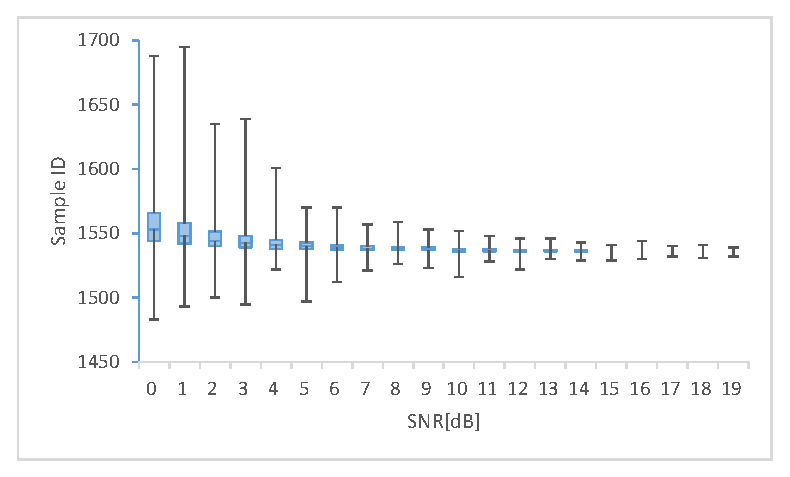
\includegraphics[width=120mm]{transition_up.eps}
\caption{Boxplot result of the rise up point.}
\label{transition_up}
\end{figure}
\begin{figure}[!htp]
\centering
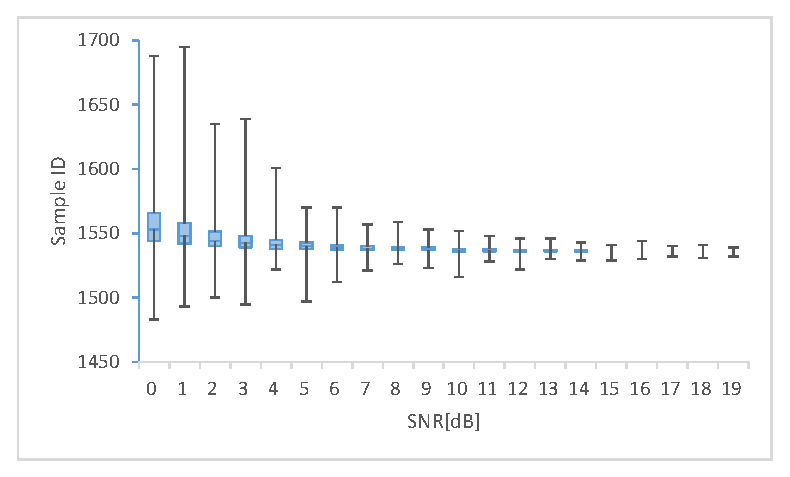
\includegraphics[width=120mm]{transition_down.eps}
\caption{Boxplot result of the rise down point.}
\label{transition_down}
\end{figure}

\begin{figure}[!htp]
\centering
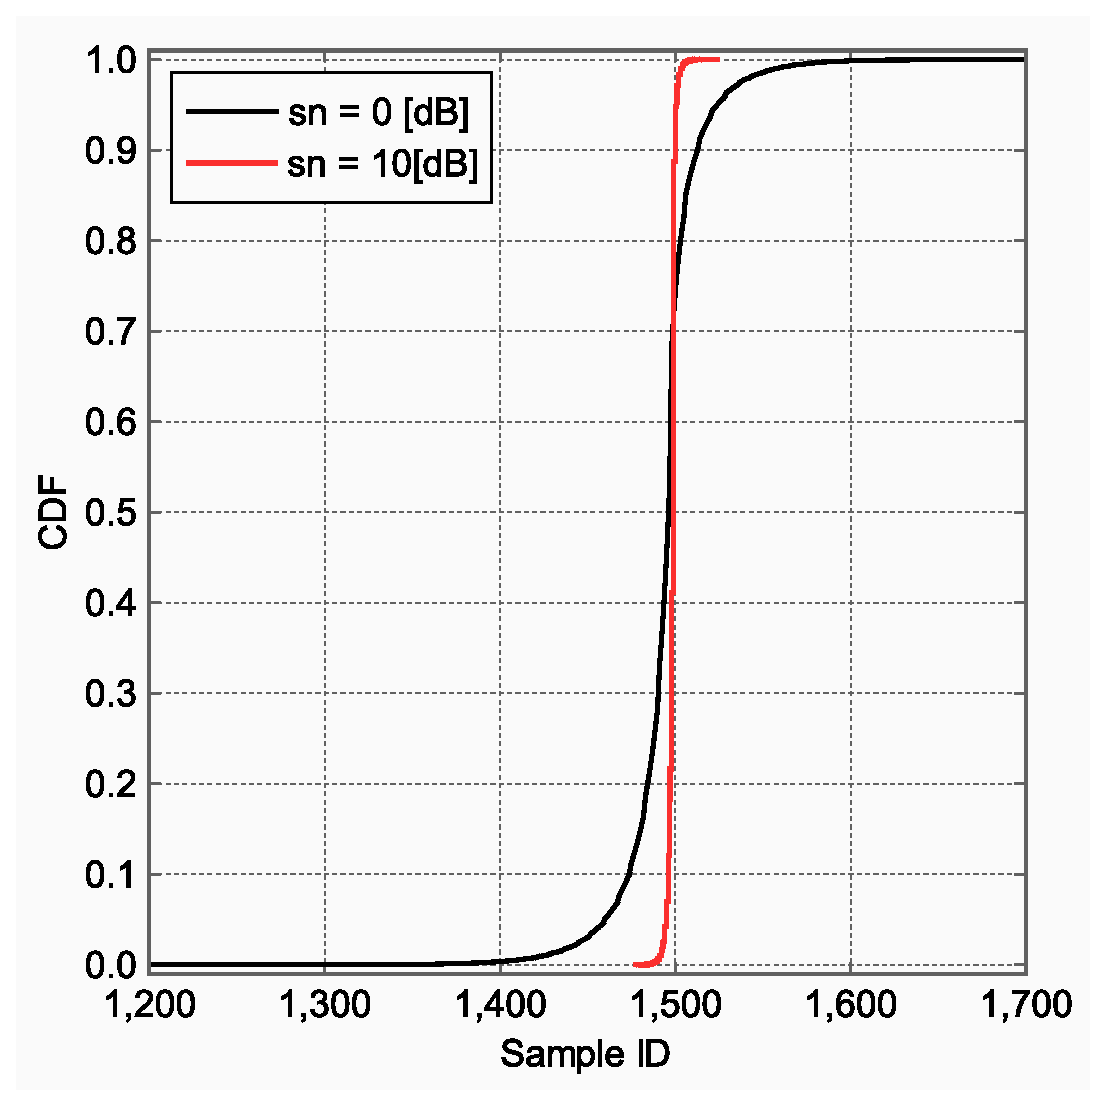
\includegraphics[width=100mm]{cdf_OFF2ON.eps}
\caption{CDF of rise up point detection(rise up point is set to be 500th sample).}
\label{cdf_off2on}
\end{figure}


\begin{figure}[!htp]
\centering
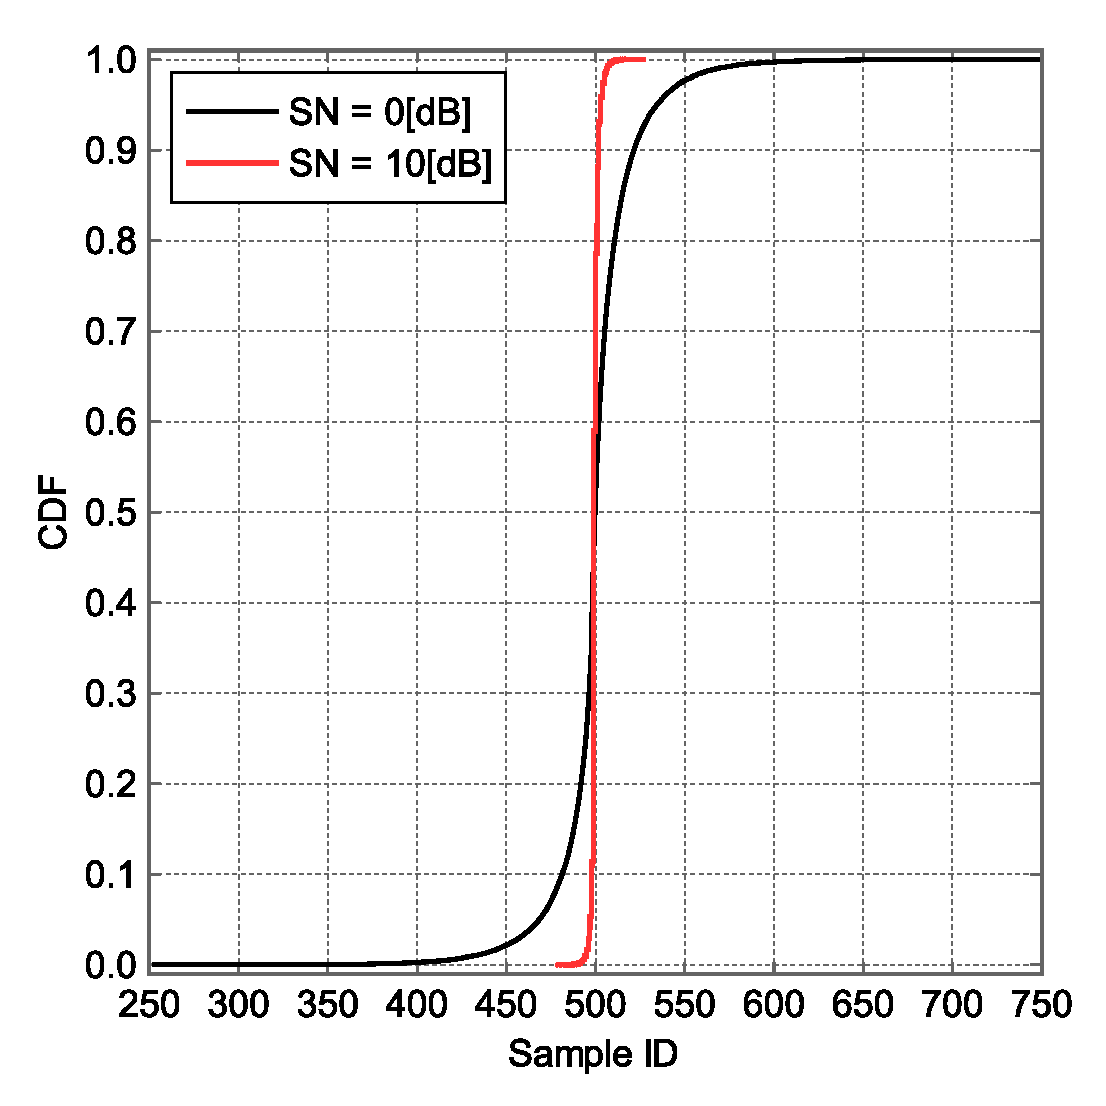
\includegraphics[width=100mm]{cdf_ON2OFF.eps}
\caption{CDF of rise down point detection(risen down point is set to be 1500th sample).}
\label{cdf_on2off}
\end{figure}

\begin{figure}[!htp]
\centering
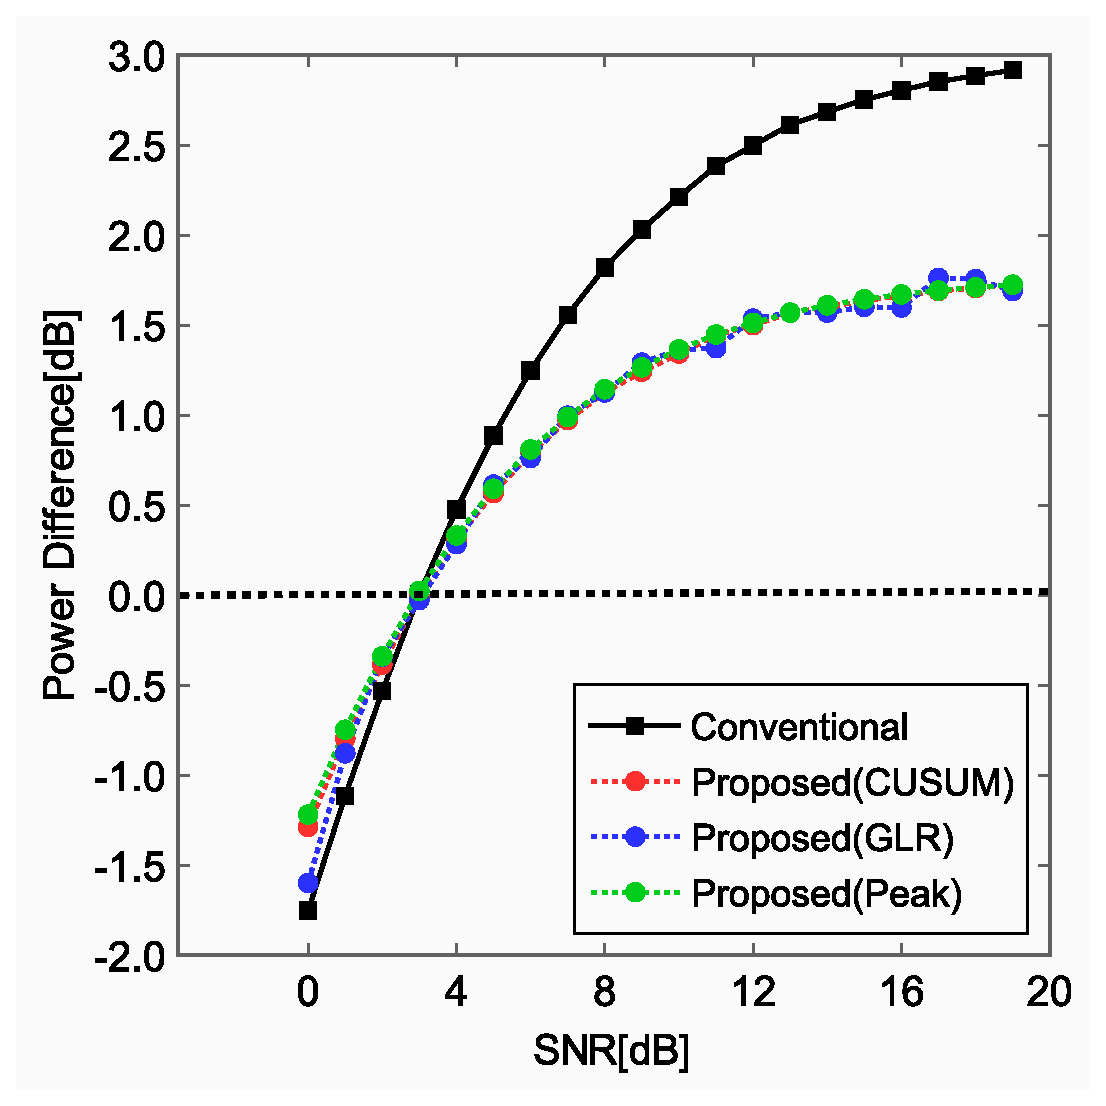
\includegraphics[width=100mm]{peak.eps}
\caption{The power difference with the real power.}
\label{Powdiff}
\end{figure}

\begin{figure}[!htp]
\centering
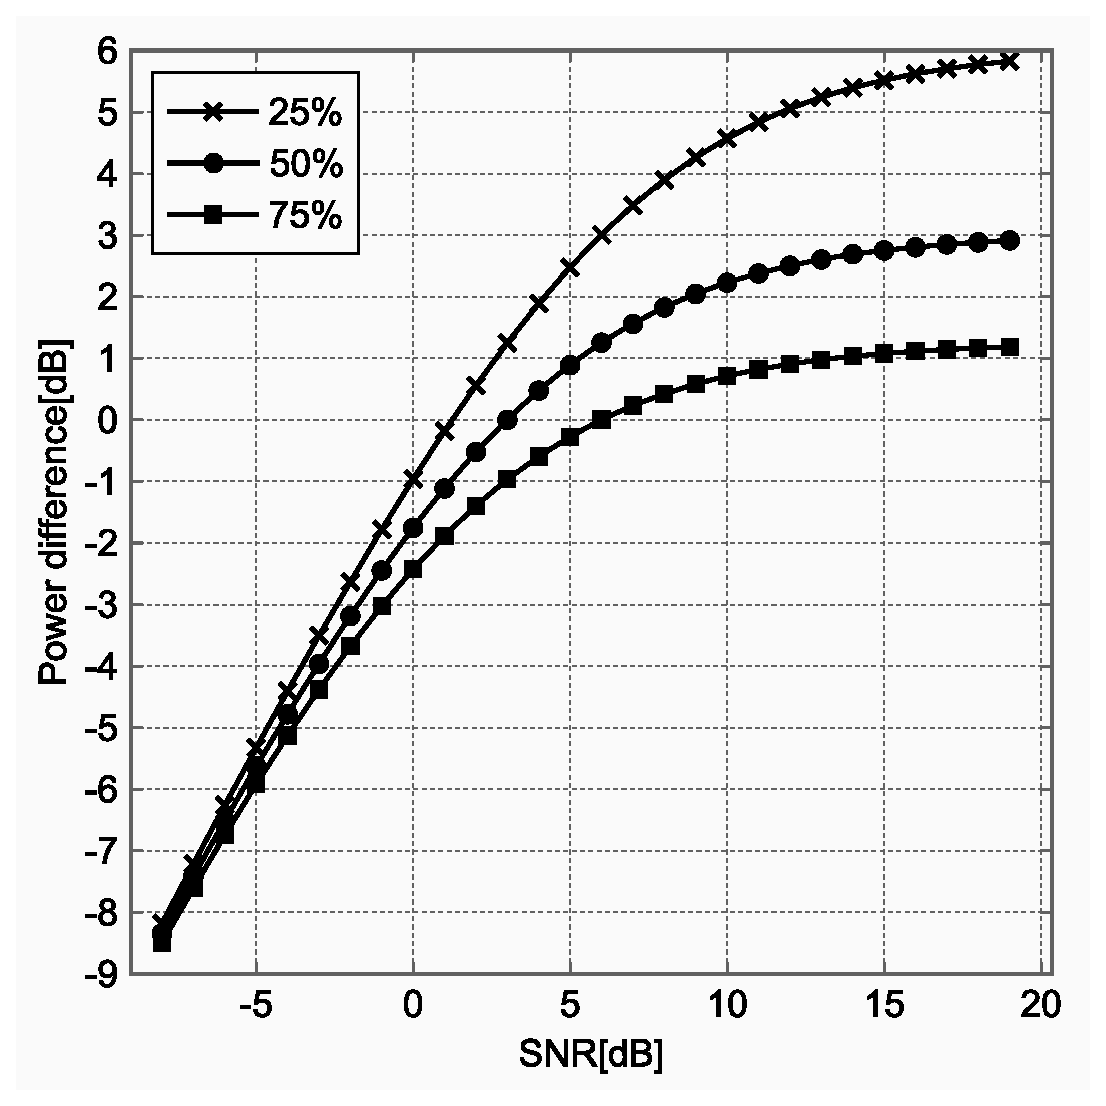
\includegraphics[width=100mm]{per.eps}
\caption{The power difference with the real power at different ON percentage during the sensing period.}
\label{per}
\end{figure}
